\section{General Discussion}

Motivated by a recent probabilistic model of scalar adjectives \cite{lassiter_context_2013}, we argued that adjectival intensifiers could gain aspects of their meaning through a systematic pragmatic inference, even in the absence of conventional literal meaning.
Our \eb{M-implicature model (presented in further detail in our \hyperref[app:model]{Appendix})} predicted a linear relationship between the intensity of an intensifier and its communicative cost, measured here in terms of length and negative log-frequency%
\eb{, and we explore this linear relationship using regression models.}

In five experiments we provided evidence that intensifier meanings do depend systematically on the length and frequency of occurance of those word forms and that this relationship holds even for novel words.

While it is unlikely that this accounts for all intensifier meaning, our results do suggest that a major portion of meaning comes not from arbitrary, conventional association of signal to sign \cite{de_saussure_nature_1916}, but from features of the word's form and distribution, together with inferential processes of listeners.

For the semantics of adverbial modifiers, we have shown how pragmatic mechanisms could be central in establishing flexible contributions to sentence meaning.
We have extended previous proposals that degree adverbs transform or create new threshold variables, providing a concrete mechanism for interpreting an arbitrary degree adverb in an arbitrary context.

This mechanism for linking a parsimonious semantics to interpretation via pragmatic inference follows naturally and straightforwardly from an understanding of rational social agents engaging in communication.
With the minimal assumption that each use of a scalar adjective has a different threshold, we have been able to extend a model of adjective interpretation to account for a major source of intensifier meaning.
This model adds to an abundance of linguistic phenomena --- e.g. aspects of metaphor \cite{kao_formalizing_2014}, prosody \cite{bergen_strategic_2015}, politeness \cite{yoon_i_2017}, and presupposition projection \cite{qing_rational_2016} --- which can be explained within the basic RSA framework, each with minimal, compatible assumptions.
The precise specification of this model is laid out in more detail in the Appendix.

Our proposal and our experiments suggest that even a very minimal semantics for intensifying degree adverbs can be plausible and productive.
We have implemented and described one version of such a semantics, but other versions might exist with different methods of generating the threshold variable for an adjective phrase.

The intensifiers we have looked at may also have other source(s) of meaning in addition to the measures of communicative cost that we have explored.
There appears to be consistent variation in intensifier meaning beyond that explained by our measures of communicative cost.
As an illustration of the remaining variance, we first averaged across participants and adjectives to get an average scaled response for each intensifier.
We then computed the squared correlation between those values and the surprisal predictor ($R^2=0.293$ for Study \hyperref[sec:study1a]{1a}, $R^2=0.273$ for Study 1b, and $R^2=0.358$ for Study 2)\footnote{
For intuition this means that one nat difference in surprisal predicts 0.128 normalized units of cost difference. In the case of laptops, for example, one nat of surprisal would predict approximately a 9\% increase in the interpreted price.
}.
% In the discussion, "This remaining variance may be because we have not exhausted the sources of communicative cost.." and subsequent: I found this part hard to follow. It almost seems like the authors are apologizing for not being able to explain all variance. It would be surprising if, in a system like language, all variance could be explained by communicative cost. We should expect some random variation. I think the authors could be clearer about what role--and how much of a role--considerations of communicative cost should play in language design.
% \eb{
% It could be that there are systematic factors affecting prices that we have not captured.
% For example, 
% % This remaining variance may be because we have not exhausted the sources of communicative cost.
\todo{be clearer about what role--and how much of a role--considerations of communicative cost should play in language design.}
% It could also be that in addition to the relationship we have described between communicative cost and strength, conventional contributions to meaning are associated with certain adverbs.
% In particular, many intensifiers seem to be derived from adverbs having to do with emotion, and the valence and/or arousal of these root emotions might influence the strength of an intensifier or its affinity to co-occur with some adjective types rather than others.
% This might be especially true for intensifiers that are still making the change from manner adverb to intensifier (e.g. terribly once only carried the qualitative meaning of ``bad and frightening'', but now almost exclusively means simply ``a lot'').

In investigating our proposal of how intensifiers get their meanings, we have collected many judgements about the relative strengths of intensifiers across several adjective scales and dependent measures.
As a summary of these judgements, we have aggregated across the different dependent measures in our studies and displayed them in a common scale in Figure~\ref{fig:intensities}.
For each study, we computed the average value of the dependent measure (normalized log-transformed price for Studies 1a, 1b and 3 and height in list for Studies 2 and 4) for each intensifier in that study. We then z-scored within the study, so that our different operationalizations of ``strength'' in the different study designs could be reasonably compared together.
Given this rescaling, we can compare the strengths of these intensifiers to one another, including the novel intensifiers from Studies 3 and 4.
We see some consistency across experiments and show that our choices of novel intensifiers spanned the full range of natural intensifier strengths.

For the broader question of form-meaning mapping, we have suggested a source of non-arbitrary association based on both properties of the word form and of its distribution.
The effect of a word's distribution on its interpretation has potentially interesting implications for language change.
If the distribution of a particular grammatical category of word (e.g. intensifiers) influences its meaning and the meaning of a word in turn influences its distribution, this would result in an unstable lexicon for this grammatical category.
This suggests a mechanism by which overused words might become stale, and would predict the rapid creation of new, unusual intensifiers.
This process indeed seems to be evident in the history of English \cite{bolinger_degree_1972}.

We have argued that form-to-meaning mapping can come about through the inferences known to support pragmatic interpretation.
Seen another way, the basic assumption that people are actively trying to communicate with each other---each reasoning about what the interlocutor means---\emph{requires} non-arbitrary relationships between a variety of factors and effective meaning.
Some systematic aspects of meaning follow directly from the principles of language understanding.

\begin{figure}[hbt]
\begin{center}
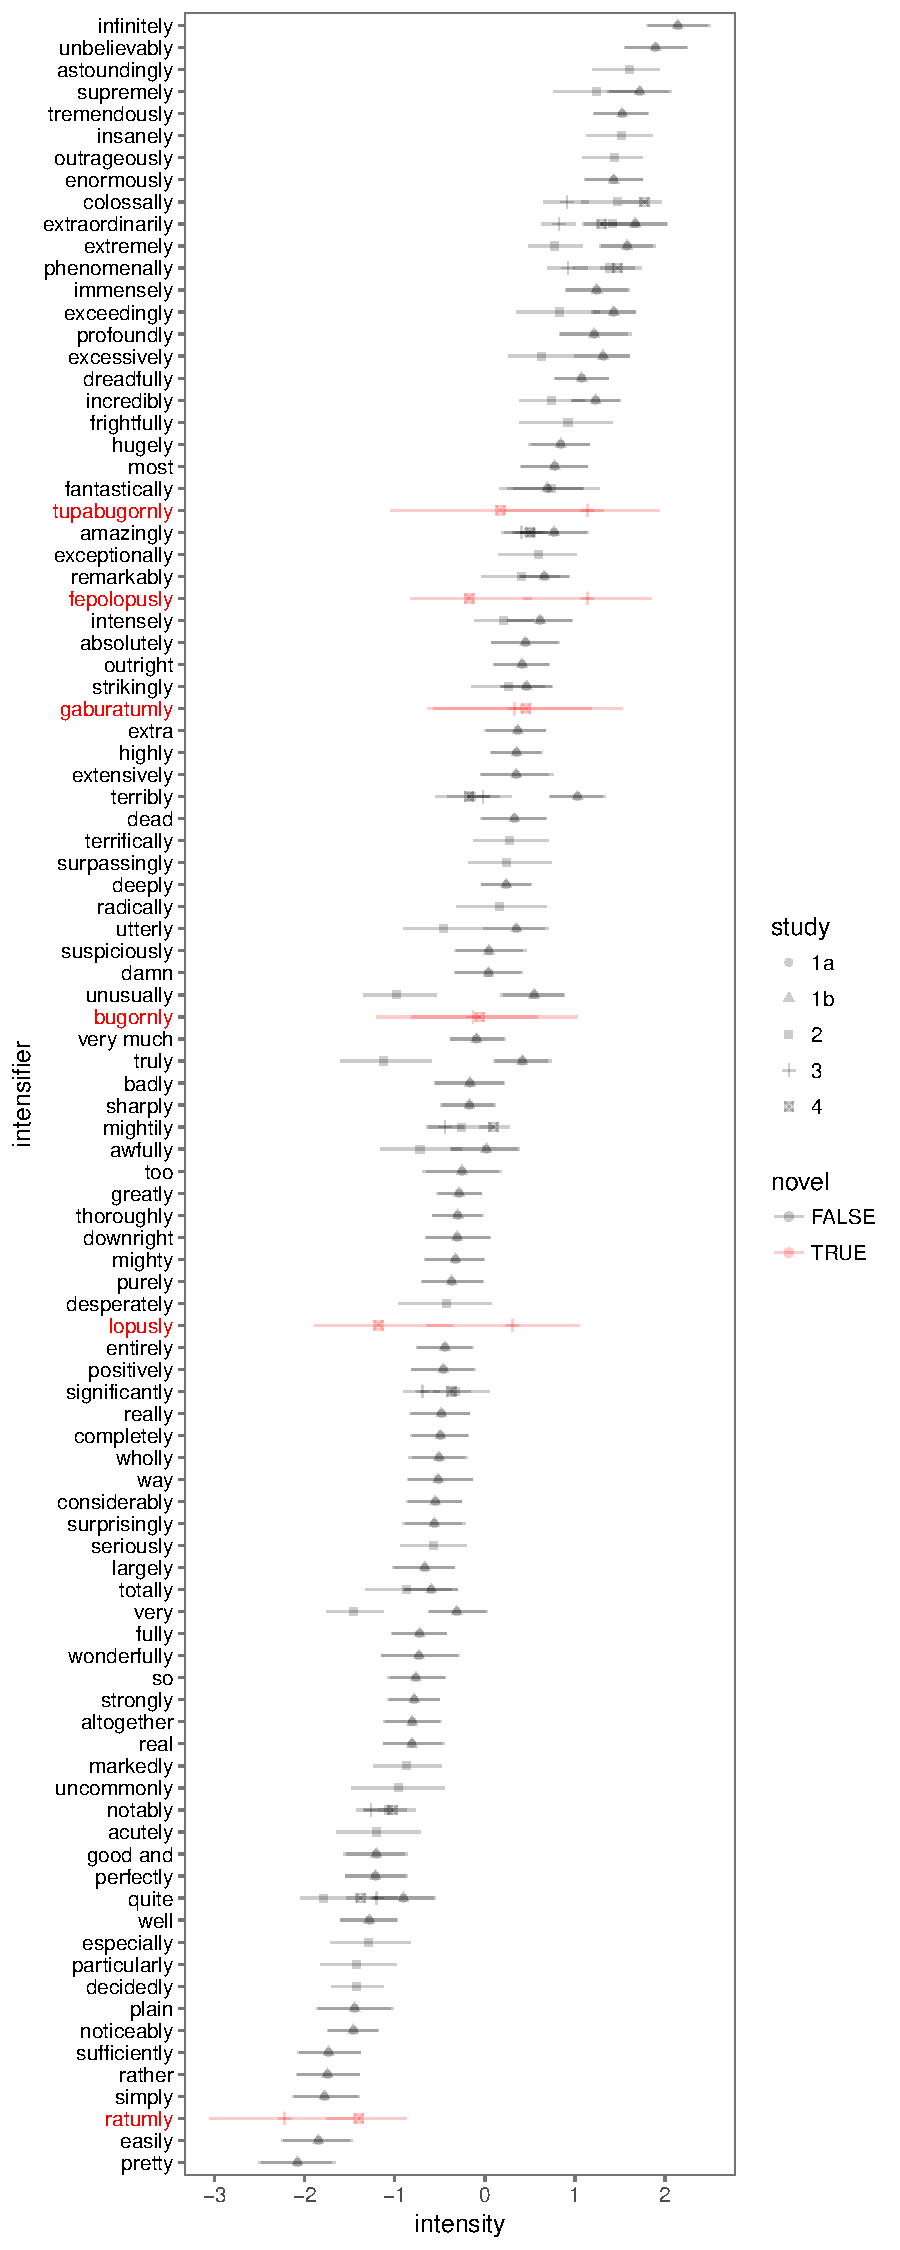
\includegraphics[width=0.5\textwidth]{images/intensities.pdf}
\end{center}
\caption{Intensities (each dependent measure, z-scored) of all intensifiers across all 5 studies. Novel intensifiers are shown in red, standard English intensifiers in black.}
\label{fig:intensities}
\end{figure}
